\documentclass{article}
\usepackage{graphicx}
\usepackage[hidelinks]{hyperref}
\usepackage{subcaption}
\usepackage{pdfpages}

\graphicspath{{./figures/}}

\begin{document}

\title{Research in VGIS - Miniproject}
\author{Niclas Hjorth Stjernholm}

\maketitle

\section{Tensorflow Playground Tasks}
\subsection{Default settings}
\subsubsection*{Circles data}
The model converges very fast, within just around 150 iterations.
The data is divided in a simple pattern, and with the given two hidden layers with four and two neurons, the pattern created from the data is learned in a fast manner. With this low a complexity of pattern only a few neurons a used to learn the pattern and to classify the data.

\begin{figure}[h]
  \centering
  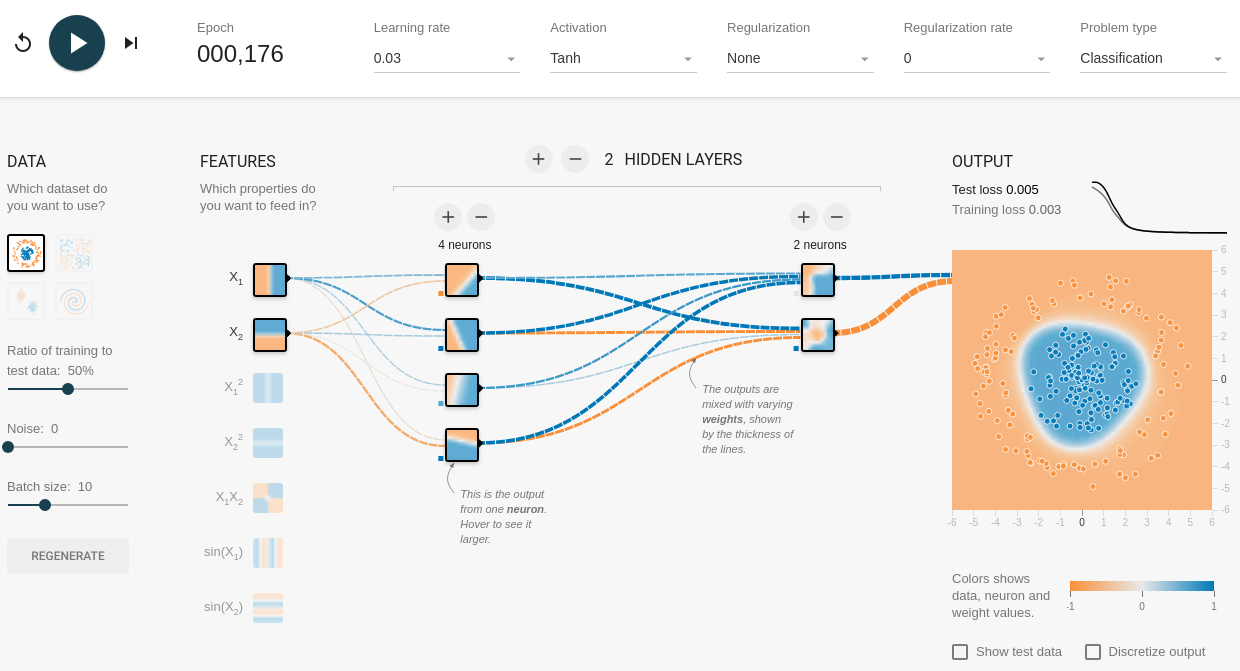
\includegraphics[width=0.8\textwidth]{default.png}
  \caption{Default settings with a disc and a circle as data}
  \label{fig:default}
\end{figure}

\subsubsection*{Spiral data}
The model has a training loss of just around $0.3$ and a test loss even higher. This points to an underfitting which means the model is not able to properly fit to the data with the given capabilities.

\begin{figure}[h]
  \centering
  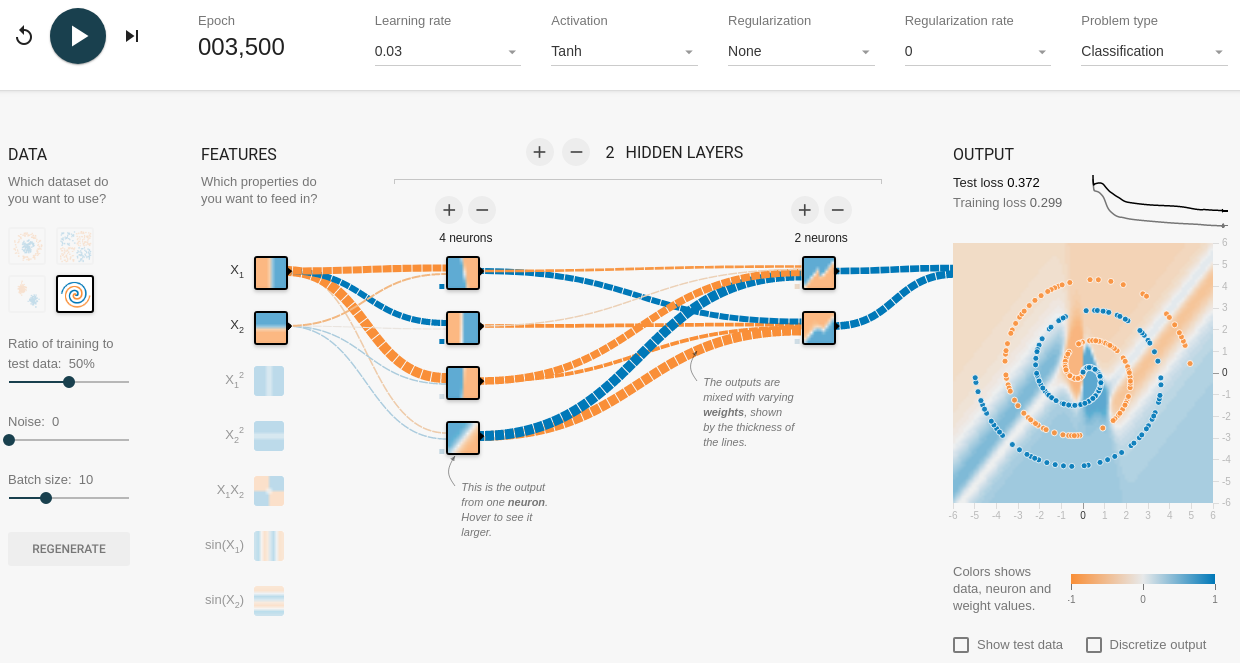
\includegraphics[width=0.8\textwidth]{default_spiral.png}
  \caption{Default settings with the spiral data set}
  \label{fig:def_spiral}
\end{figure}

\subsection{altered settings}
By increasing the amount of neurons to eight and adding another layer with six neurons, the model is able to converge to the data and attain a fitting shape. The only other thing changed is the learning rate, changed from $0.03$ to $0.01$.

\begin{figure}[h]
  \centering
  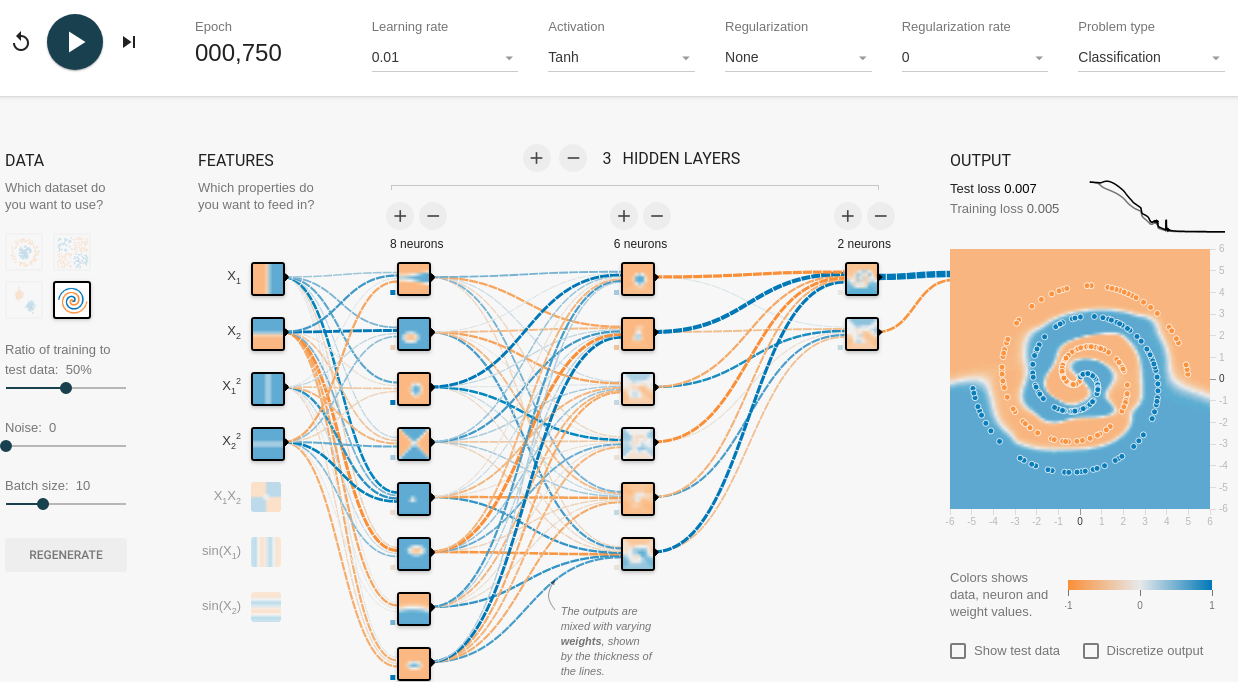
\includegraphics[width=0.8\textwidth]{alternated_spiral.png}
  \caption{Altered settings with the spiral data}
  \label{fig:alt_spiral}
\end{figure}

As seen in \autoref{fig:alt_spiral}, by adding the features $X_1^2$ and $X_2^2$ the model is able to form more complex outputs in the neurons.\\
With more neurons in the first hidden layer the model is once again able to generate higher complexity and by that weighting of the outputs to the next layer. With the extra layer with six neurons we are able to create more complex outputs, as seen in the figure. It is clear how the bottom neuron in the second hidden layer is already closing in on making a spiral. In the third hidden layer with just two neurons, it is again clear that a spiral is created, and the one closer to the spiral has a much higher weight than the other neuron output.

\subsubsection{Adding Noise}
When adding noise the model starts to break and is unstable at a noise level of 30. \autoref{fig:noisefigs} shows the the stable model at noise level 25 and the unstable model at noise level 30.

\begin{figure}[h]
  \centering
  \begin{subfigure}[b]{0.48\textwidth}
    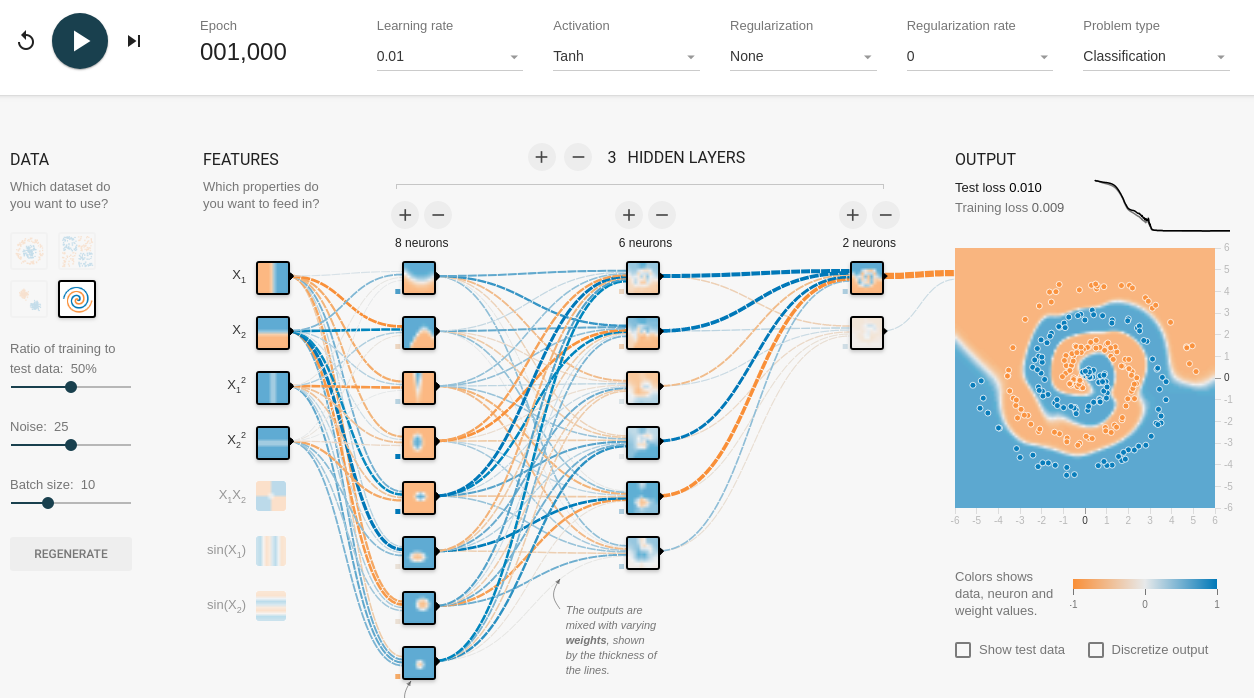
\includegraphics[width=\textwidth]{altered_noise_25}
    \caption{Altered settings with the spiral data, adding noise at a level of 25}
    \label{fig:alt_noise_25}
  \end{subfigure}
  \hfill
  \begin{subfigure}[b]{0.48\textwidth}
    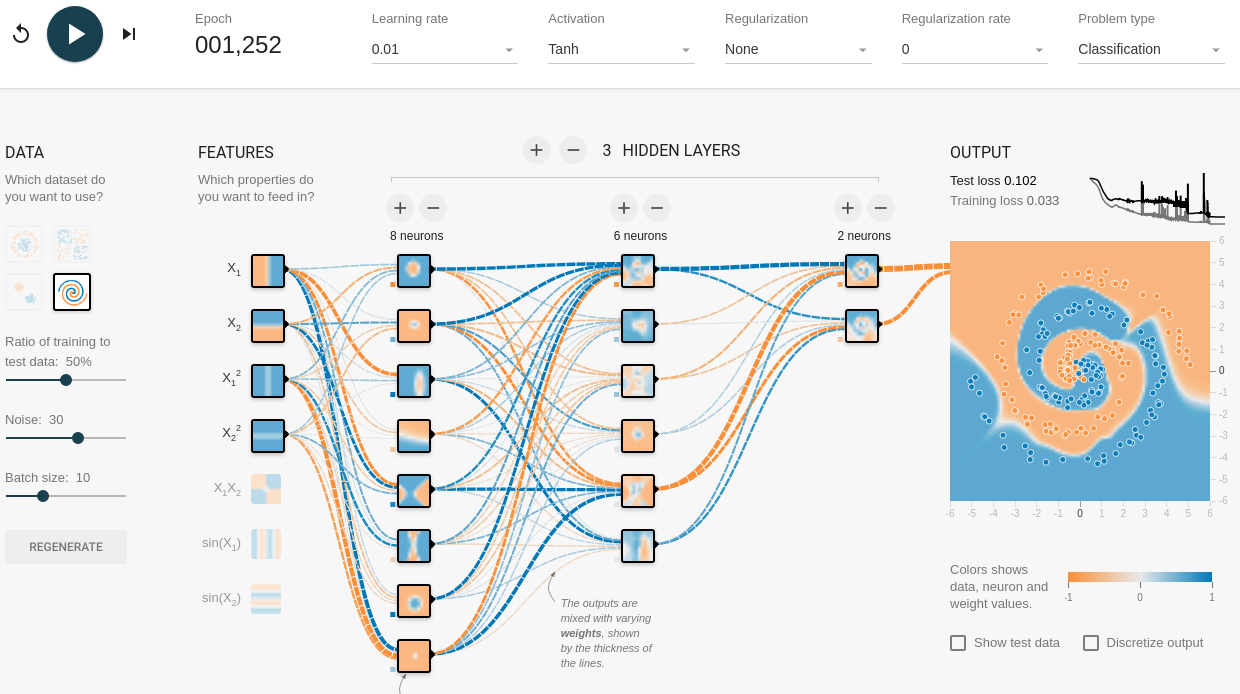
\includegraphics[width=\textwidth]{altered_noise_30}
    \caption{Altered settings with the spiral data, adding noise at a level of 30}
    \label{fig:alt_noise_30}
  \end{subfigure}
  \caption{The two models with added noise}
  \label{fig:noisefigs}
\end{figure}

\section{Quick, Draw! Doodle Recognition Challenge}
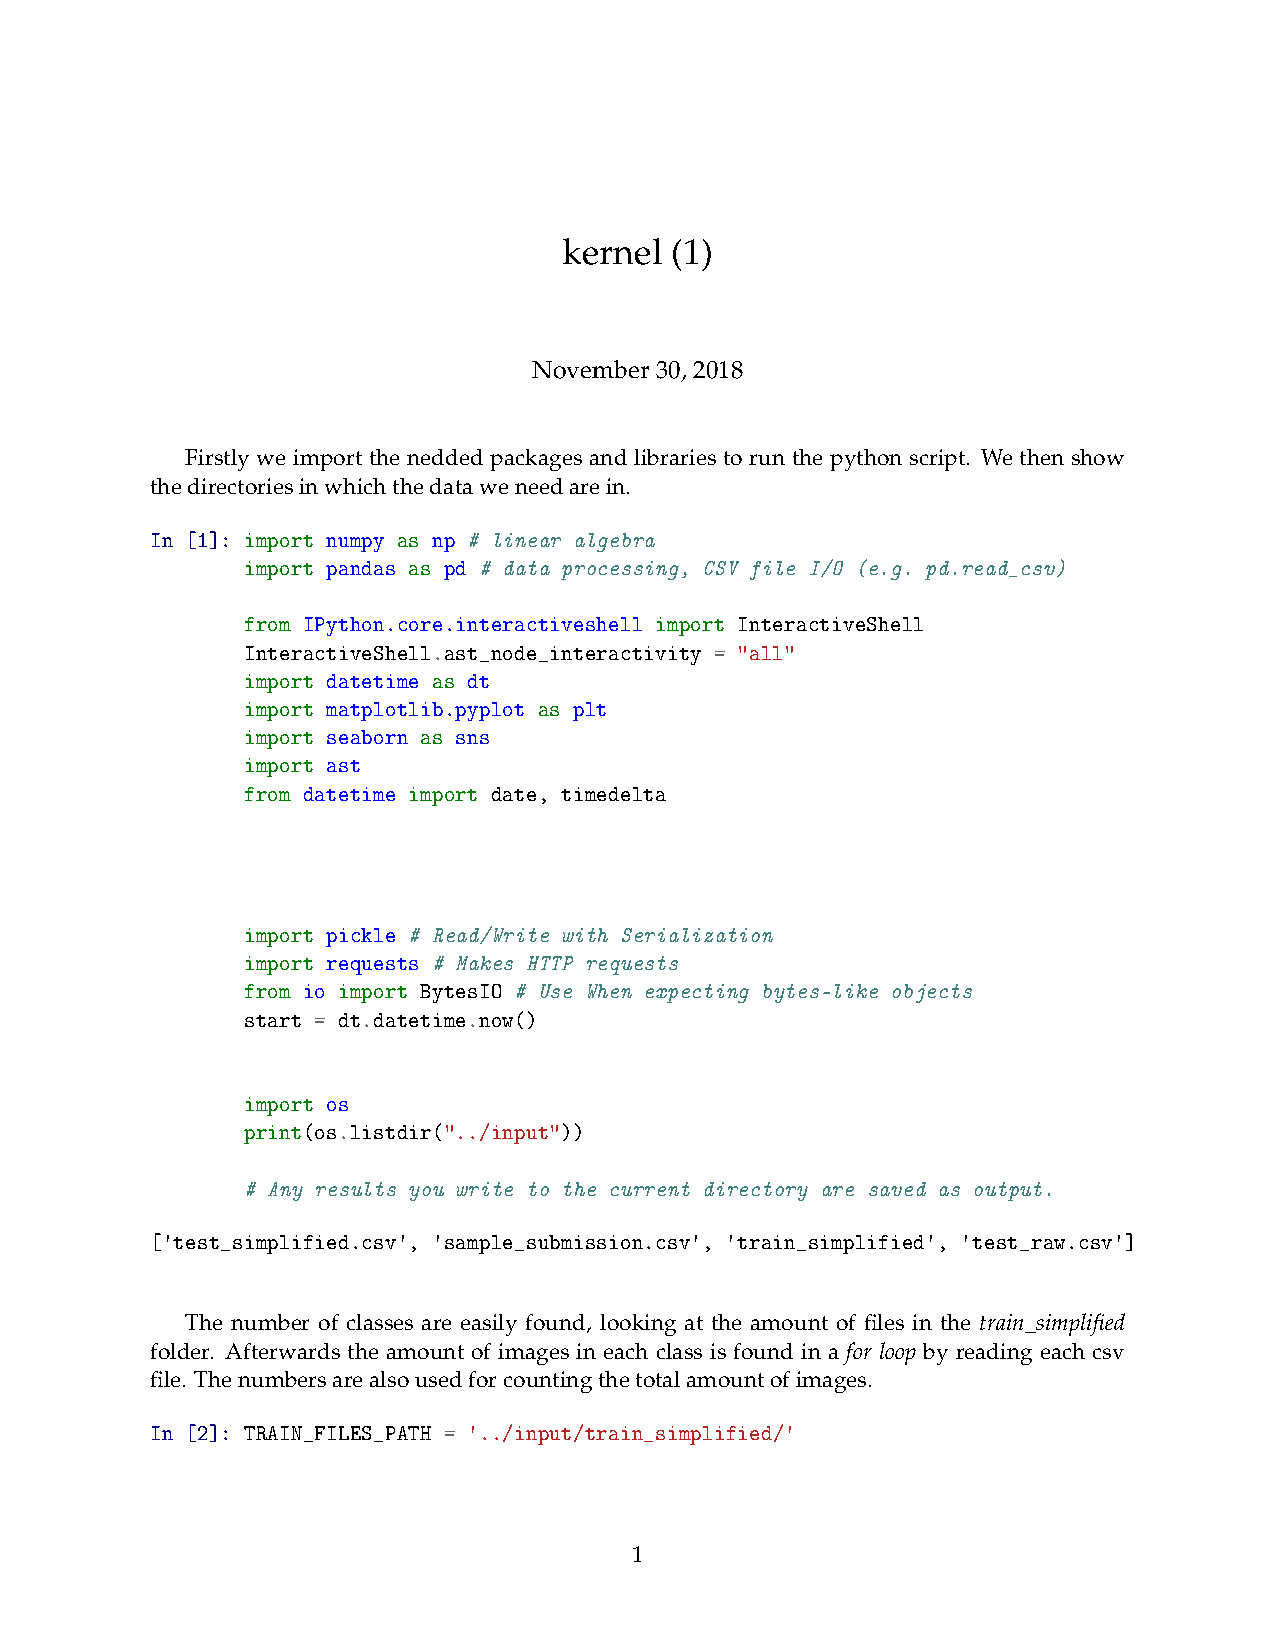
\includepdf[pages=-]{kernel.pdf}
\end{document}
